% A template for master's thesis, W.H. 2006
% If your superviser wants an another template, use it!
% This file contains only the cover page and all chapters are in 
% different files
\documentclass[a4paper,12pt]{book}

%useful special symbols:
%\usepackage{amssymb}
\usepackage{latexsym}
\usepackage{graphicx} 
%\usepackage{CJK}
%\usepackage{pinyin}
%\usepackage{tocvsec2}
%\begin{CJK}{UTF8}{cyberbit}
%a useful package if you write url addresses:
%\usepackage{url}
\usepackage{amssymb}
%\usepackage[pdftex]{graphicx} \DeclareGraphicsRule{*}{mps}{*}{} 
\usepackage{hyperref}
\hypersetup{
    bookmarks=true,         % show bookmarks bar?
    unicode=false,          % non-Latin characters in Acrobat’s bookmarks
    pdftoolbar=true,        % show Acrobat’s toolbar?
    pdfmenubar=true,        % show Acrobat’s menu?
    pdffitwindow=false,     % window fit to page when opened
%    pdfnewwindow=true,      % links in new window
    colorlinks=true,       % false: boxed links; true: colored links
    linkcolor=black,          % color of internal links
    citecolor=green,        % color of links to bibliography
    filecolor=magenta,      % color of file links
    urlcolor=cyan           % color of external links
}
%a package for figures:
\usepackage[dvips]{color}
\usepackage{epsfig}
\usepackage{booktabs}
\usepackage{listings}
\lstset{language=C++}
\lstset{tabsize=4}

%Default for bibliography style. The alpha style generates references with 
%first letters and year. If your supervisor asks another style, change this. 
%\bibliographystyle{alpha}


%Create your own environments
\newtheorem{definition}{Definition}
\newtheorem{example}{Example}

%if you want to use multicolumn tables, uncomment the following:
%\usepackage{multicol}
%if you want to use sideway tables or figures, uncomment the following:
%\usepackage{rotating}x1

%The following packages are needed e.g. for algorithm environment
\usepackage{float}
\usepackage{algorithmic,algorithm}
\usepackage{xspace}
\usepackage{mathptmx}
%Uncomment to include algorithm environment (you need file algorithmwh.sty):
\usepackage{algorithmwh}

\textwidth=14.945cm
\oddsidemargin=0.5cm
\evensidemargin=0.5cm

%By default, each paragraph begins by an indent (space). If you prefer
%no indent but an empty line between paragraphs, uncomment the following: 
%\setlength{\parindent}{0pt}
%\setlength{\parskip}{1.5ex plus 0.5ex minus 0.2ex}
 
%%%%%  

\begin{document}

%the title page begins
\begin{titlepage}

\vspace{3cm}


\noindent
%\begin{flushleft}
\setlength{\baselineskip}{2\baselineskip}
\begin{center}
{{\Large \bf Implementation of Bit-Stream based on P2P overlay network }}

\vspace{1cm}
A Thesis Submitted to \\
Nanjing Normal University\\
For the Academic Degree of Master Engineering \\
\end{center}

%\end{flushleft}

\newcommand{\TitleStyle}[1]{{\Large \textbf{#1}}}
\newcommand{\TitleSpace}{\vspace{2pt}}
\vspace{2cm}
\noindent
{Author by: \bfseries{\emph{Xiang Wang}}\\
\itshape{Supervised by} : Assoc.Prof. \bfseries{\emph{Ziyv Zhang}}}

\vspace{1cm}
\vspace{\fill}
\vspace{2cm}
\begin{tabbing}
mmmmmmmmmmmmmmmmmmmmmmm\= \kill
\>Master's thesis \today\\
\>Department of Computer Science\\
\>Nanjing Normal University\\
\> \\
%%\> \\
\end{tabbing}
\end{titlepage}
%the title page ends

%%%%%
\thispagestyle{empty}
%Abstract
\newlength{\origpar}
\setlength{\origpar}{\parindent}
\setlength{\parindent}{0pt}
%A template for the abstract

\begin{center}
{\large \bf Implementation of Bit-Stream based on P2P overlay network}\\
\end{center}
Xiang Wang\\

Department of Computer Science\\
122 Ninghai Road, Nanjing, 210097, Jiangsu Province\\
Master's thesis\\

\begin{center}
{\bf \emph{Abstract}}\\
\end{center}
{\hspace{1cm}There is no doubt that Video-on-Demand \emph{(VoD)} nowadys is one of the most popular Network Applications on the Internet, contributing to a significant portion of the Internet traffic and being a basis usage of \emph{P2P Internet Protocol} emerging services.
However, with current P2P swarming systems were based on Bit-torrent algorithm, so one or much many central tracker servers were necessary to be deployed in the  open Internet. In this half-centralized P2P system, it was hard to avoid \emph{DDoS} attacking. 
A lot of effort has gone into optimizing the distribution of large files and media in BT-liked P2P system, 
little research has been done on enabling Bit-Stream functionality with P2P swarming systems based on \emph{Kademlia} algorithm . The main challenges reside in ensuring
that users can start watching a movie at any point in time, with small start-up times and sustainable playback rates, and can effectively avoid \emph{DDoS} attacking, which will ensure the performance of VoD service.\\
\hspace*{1cm}{}In this work, this paper address the issues of providing Bit-Stream using P2P \emph{kademlia-based} networks and \emph{OGG} decode containner. This paper investigate scheduling techniques, and network coding in particular. 
Using both simulations and a prototype implementation,
{\footnote{\it{I have set up a project with the name of \emph{KadPeer} in code.google} with GPL2 license. 
(\url{http://code.google.com/p/kadpeer/}). Source code can be downloaded freely.}} 
it shows that high-quality VoD is feasible, 
and give guidelines to build play-as-you-download P2P swarming systems with low start-up delays.
%In this work, we build analytical models to capture
%the performance of BitTorrent-like P2P systems in a steady state, in the presence
%of homogeneous and heterogeneous NAT peers. 
I also build analytical models, in order to improve the overall system performance and fairness
ivmetrics considerably. The analytical models have been validated by simulation results,
which also reveal some interesting facts about the coexistence of NAT and public peers
in \emph{Bit-Stream} systems.}
\vspace*{1cm}

%List keywords here
{\bf Key words}:\it{\emph{ Bit-Stream; VOD; P2P; kademlia; OGG}}\\
%{\bf Computing Reviews (2010) Categories and Subject Descriptors:}\\
%List the classes here.\\
%The following is optional


\setlength{\parindent}{\origpar}

%if you want to include acknowledgements, uncomment the following:
%\thispagestyle{empty}
%input{acknowledgement}
%Now the file is called acknowledgement.tex
\thispagestyle{empty}
\tableofcontents
\clearpage
\pagebreak 
\renewcommand {\baselinestretch} {1.389}
\linespread{1.5}
\pagenumbering{arabic}
%\bibliographystyle{plain}
%\bibliography{refs.bib}

\chapter{Introduction}
\label{Introduction}
{This is an overview of the main techniques of media streaming in the past years. It interpretes the phylogeny of media content delivery system, which includes from the traditional client-server framework to the Peer-to-Peer mesh network topology based delivery method system. And also, it will contain the main extra knowledge about P2P system and video media encapsulation techniques, which was widely used in current media player codec software , such as Gstreaming, VLC, and many other open source softwares.}

\section{Traditional C/S Architecture based Streaming}
{
  Traditional C/S Architecture based media content delivery system, which once occupied a high rate market share in old days, has its advantages in many points. Because of its centralised resources management and server level administration, many applications were designed and implemented in this kind of network environment. Thanks to this architecture it is possible to remove or add clients without affecting the operation of the network and without the need for major modification.

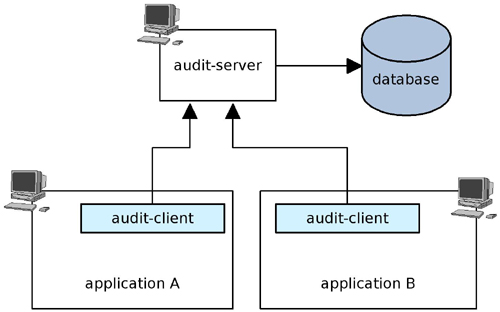
\includegraphics[width=10cm]{data/architecture-small.jpg}
\\

However, due to the technical complexity of the server, the sever will be the only weakness in this architecture. The large number of clients access the same server, which will lead to traffic congestion, that directly affects the performance and fault-tolerance requirment of video delivery system.

In traditional C/S model, all of the media data interchangement should involve server machine, as the growth of client quantity, server will become the bottleneck of whole video delivery system. Once the Server crashed, and the whole system will crashed as well. Secondly, C/S based video delivery system totally depends on the central node -- server. It can not work without server node, and then it will be meaningless of the whole network. Thirdly, there are a great volume of idle resources in client end (such as disk usage, CPU circle). If the client dose not get the response from server, all of the resurce will be dissipated. This will absolutely lead to a low resource utilization.
}

\subsection{RTP/RTSP protocol based live Video Streaming}
{
RTP is a transport protocol for the delivery of real-time data, including interactive streaming audio and video under single broadcast or group multicast environment. 
Applications usually run RTP based on UDP protocol, in order to mux the usage of multi-node and inspection services;even both of the two protocols contain the transport layer protocol functions.
However, RTP can be integrated with the other suiteable underlying netork or transport protocol. 
If the underlying network support group multicast service , RTP can use the multicast table to deliver the data to multiple destinations.

RTP does not support delivering on time mechanism or any other \emph{QOS} assurance. That means RTP can not ensure avoiding disorderly transfer or the reliability of the underlying network. However, RTP is a orderly transfer protocol. The Serial Number in RTP transfer session enabled the recipient to restruct the serial packages.

RTCP is a part of RTP and helps with lip synchronization and QOS management, among others, which also can provide the infomation about transfer members in the session. The second aspection of RTCP functions is enough for \emph{Loosely controlled} session, that means, if there is no specific memeber to control or orgnize, it does not have to be used as an application which can control all of the communicate requests.

\begin{center}
\begin{tabular}{@{}llllll@{}}\toprule
1   & 2 &   3 &   8             &           9      & 16bit\\\midrule
V 	& P &   X &   CSRC Count 	&           M 	   &Payload Type\\
\multicolumn{4}{c} {Sequence number}               &  Timestamp\\
\multicolumn{4}{c}{SSRC} 	    &\multicolumn{2}{{c}}{CSRC (variable 0 – 15 items 32bits each)}\\
\bottomrule
\end{tabular}
\end{center}
\footnote{The table indicates RTP package elements, more detail information can be refered in RTP wiki page \url{http://en.wikipedia.org/wiki/Real-time_Transport_Protocol}}
\begin{itemize}
\item V -- Version,indicates the version of the protocol.
\item P -- Padding,used to indicate if there are extra padding bytes at the end of the RTP packet.
\item X -- Extension,indicates presence of an Extension header between standard header and payload data.x
\item CC --Contains the number of CSRC identifiers (defined below) that follow the fixed header.
\item M -- Marker,Used at the application level and defined by a profile.
\item PT -- Indicates the format of the payload and determines its interpretation by the application. 
\item SN -- Sequence number,incremented by one for each RTP data packet sent and is to be used by the receiver to detect packet loss and to restore packet sequence.
\item TT -- Timestamp ,Used to enable the receiver to play back the received samples at appropriate intervals.
\item SSRC -- Synchronization source identifier uniquely identifies the source of a stream. 
\item CSRC -- Contributing source IDs enumerate contributing sources to a stream which has been generated from multiple sources.
\end{itemize}

RTSP is a control protocol that initiating and directing delivery of streaming multimedia from media servers, the "Internet VCR remote control protocol". 
RTSP does not deliver data (though the RTSP connection may be used to tunnel RTP traffic for ease of use with firewalls and other network devices). 
The proposed standard of RTSP has been defined in RFC2326, which was widely used in media stream transmission. At present, most of the resolvents on real and quick time media stream are support RTSP protocol.

The design and implement of RTSP is similar to HTTP protocol. The relationship between RTSP and RTP/RTCP is familar with the one between HTTP and TCP. But still, there is much diversity. RTSP is a durable link in the process of media stream dibbling and palyback. So, no matter Client or Server can have a state. However, there is no state in HTTP protocol; HTTP status information needs other ancillary mechanism to maintain,such as \emph{Cookie}. In addition, RTSP does not use the RTP / RTCP, but to manipulate them, and itself is still using the TCP protocol. The HTTP uses TCP transport.
Demand that the entire media and playback process is a Session, Session embodies a state machine, Client and Server have a state machine each.

The state machine of client are as followed, and the events are receiveed from user input.
\begin{center}
\begin{tabular}{@{}lll@{}}\toprule
                    &       EVENT                &    TARGET \\ \midrule
                    &       TEARDOWN             &     Init\\  
   Init             &       SETUP                &      Ready \\ \midrule
   Ready            &       PLAY                 &      Playing \\
                    &       RECORD               &     Recording\\
                    &       TEARDOWN             &      Init\\
                    &       SETUP                &      Ready\\\midrule
   Playing          &      PAUSE                 &      Ready\\ 
                    &     TEARDOWN               &      Init\\
                    &      PLAY                  &      Playing\\
                    &     SETUP                  &      Playing \\\midrule
   Recording        &      PAUSE                 &      Ready\\ 
                    &     TEARDOWN               &      Init\\
                    &     RECORD                 &      Recording\\
                    &      SETUP                 &      Recording \\\bottomrule
\end{tabular}
\end{center}
The Serve state machine also contains the four states, state transition rules are the same, but the object and the semantic differential.
As reference HTTP, The text format of RTSP protocol is similar to the HTTP's, accurate to say that should be used in rfc822. every line of text separated by a CRLF.

}
\subsection{MMS Protocol based Video Streaming}
{

Microsoft Media Server (MMS) is the name of Microsoft's proprietary network streaming protocol used to transfer unicast data in Windows Media Services (previously called NetShow Services).\footnote{\url{http://en.wikipedia.org/wiki/Microsoft_Media_Server}}
If the audience in Windows Media Player to connect to the typed URL, rather than through a hyperlink to access the content, they must use the MMS protocol to reference the stream. When using the MMS protocol to connect to the distribution point, you can use 'protocol rollover' to get the best connection. While trying to use MMSU to connect the client point,"Protocol rollover" begins to take over the original connection. MMST is the combination of MMS protocol UDP data transfer. If MMSU connection is not successful, the server will attempt to use MMST. 
MMST is the MMS protocol with TCP data transfer.

If connected to the indexed Asf file, and you want to do fast forward, rewind, pause, start and stop the stream, you must use MMS. That was because UNC paths can not do fast forward or backward.
When connecting to the distrituted points with independent Windows Media Player, you have to specify the unicast content of URL. 
}


\section{P2P Architecture based Streaming}
{
  As the development of the information network, the demand of stream media is growing.  However, most traditional stream media service uses C/S mode,which connects to each client with unicast method. Because streaming media service is with high bandwidth and long duration, as the number of clients growing, the resource of server will be consumed very soon, which then becomes the bottleneck of whole system. As to these problems, the main solution recently is to use content dilivery network (\emph{CDN}) , and IP muiltcast. The main tech of CDN is to use proxy server which can copy the media data ,and deliver them to multiple destinations. However, this tech requres high cost, which still be the most important defect to deploy CDN in the global. As to IP multicast,because of the limitations of its own (such as hardly implementation of QOS of multicast,control of congestion, and complexity of the protocol), IP multicast is not wildely used. P2P overlay network  brings a new solution to media streaming. In the Peer to Peer network, each peer entity takes role of both server and client , which distributes the load of server to each peer. So it balances the load of the server and reduces the usage of network bandwidth ,which improved scalability of the whole system.
}

\subsection{Framework of P2P media streaming}
{
According to the way of source node delivering data, P2P media streaming system can be categorized as two types: single-source P2P media streaming transmission and multi-sources media streaming transmission. 

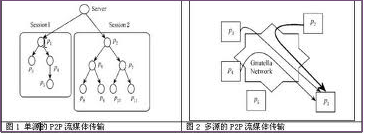
\includegraphics[width=8cm]{data/P2Pframework.png}

Single-source P2P media streaming transmission is based on application layer multicast tech, which is a tree-based multi-layer structure. 
There is a single source sender and multipule data receivers, and each receiver acquires data only from one sender. The server and all of the peer nodes make up of a multicast tree structure. 
The node of the multicast tree receives data from its father node, and then deliver the data to its child-nodes with multicast method. 
In this structure, each client machine only acquires data from the up level nodes, so the up level nodes affect the performance of the whole system more directly. 
However, the users in the internet can not assure the quality of service, so it will be hard to maintain a stable tree-based structure. 
More over, due to the limitation of the client machines, the growth of new users which directly leads to the increasing level of the tree structure, will bring up the delayer time of the leaf machines. And the leaf nodes does not service the up level machines, so the  system can not take full advantage of the network resources.

The structure of multi-sources media streaming system is netted texture. Multipule senders transmit the data to the same receiver. Each client acquries data from multipule clients or servers segregatedly. 
The data in the buffer is divided into chunks that is with the same size. And the client sends data requests to multipule clients to acquire specify data chunk, according to a certain policy. 
In this way, the speed of data delivery can be promoted in a short time. However , this technique is complex , which involve the way to chosse sender peer, coordinate the transfer rate of multipule sender peers, and the way to allocate data segment on specific sender peers.
}

\subsection{Techniques of P2P media Streaming delivering}
{
 At present, there are two types of P2P media streaming delivering techniques:
\begin{enumerate}
\setcounter{enumi}{0}
\item Tree-based protocol and extensions. In this mode, the nodes will be organised as a multicast tree. The parent node in the tree will take responsibility for delivering media data. More attention will focus on the construction and balance of the multicast tree.
\item Gossip-based protocol. Gossip algorithm is the most popular in P2P system for delivering message. In a typical \emph{Gossip} algorithm, node will send messages to some of the nodes according to a random list, and the nodes received data will deliver the messages to the other nodes. Repeat this process , until the message has been received by all of the nodes in this P2P system. 
The media streaming system based on \emph{Gossip} algorithm does not construct the topology between nodes exhibitly, but maintain the view between each node and the some of the other nodes though the \emph{Gossip} algorithm. 
Each node will exchange the cached infomation with the other nodes, and exchange the media data according the cached infomation. In this kind of system, more buffer and more waiting time for system setting up will be required.
\end{enumerate}
}

\section{OGG Vobis bitstream encapsulation}
{
  The \emph{OGG bitstream} format has been developed as a part of a larger project aimed at creating a set of components for the coding and decoding of multimedia content (codecs) which are to be freely avaliable and free re-implementable, both in software and in hardware for the computing community at large, including the Internet community.\cite{oggencapsulationformat}. More Glossary of terms and abbreviations, please refer to Appendix A which is a part of RFC3533.
}
\subsection{The Ogg bitstreaem format} 
{
The physical Ogg bitstream is composed by multiple logical bitstreams which is so-called "Pages".  
The logical bitstreams are identified by a unique serial number in the header of each page of the physical bitstream.  
This unique serial number is created randomly and does not have any connection to the content or encoder of the logical bitstream it represents. \cite{oggencapsulationformat}  
The data of each Ogg page is unique, beacause it belongs to specific one logical bitstream only. 
And the size of ogg pages are variable, which contains header encapuslation and error recovery infomation.
Each logical bitstream in a physical Ogg bitstream starts with a special start page (bos=beginning of stream) and ends with a special page (eos=end of stream).The bos page contains information to uniquely identify the codec type and MAY contain information to set up the decoding process. The format of the bos page is dependent on the codec and therefore MUST be given in the encapsulation specification of that logical bitstream type. \cite{oggencapsulationformat}


There are two types of multiplexing of \emph{Ogg}: Grouping and Chaining.
Grouping deines the way to interleave multipule logical bitstreams in the same physical bitstream.
Chaining on the other hand, is define to concatenate physical ogg bitstreams.
In grouping, all bos pages of all logical bitstreams should appear at the beginning of the Ogg bitstream.But all of eof pages are not required to appear at the end of this streaming.
In Chaining, there is not overlap of each bitstreams. However, the chained bitstream should contain a unique serial number within the scope of the physical bitstream.
}

\subsection{The ogg page format}
{
The Ogg page header has the following format:

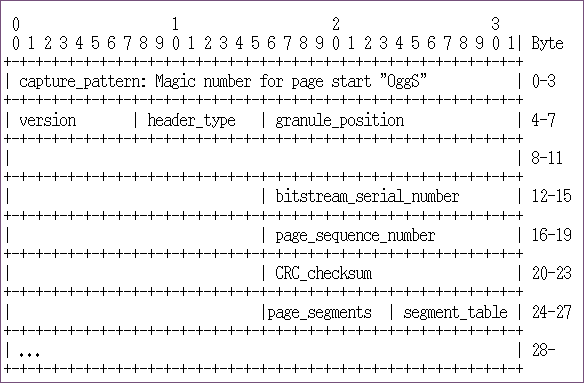
\includegraphics[width=12cm]{data/oggpageheader.png}       

\begin{itemize}
\item capture pattern -- a 4 Byte field that signifies the beginning of a
       page.  It contains the magic numbers:
             0x4f 'O'
             0x67 'g'
             0x67 'g'
             0x53 'S'
\item stream structure version -- 1 Byte signifying the version number of the Ogg file format used in this stream
\item header type flag -- the bits in this 1 Byte field identify the specific type of this page.
\item granule position -- an 8 Byte field containing position information.
\item bitstream serial number -- a 4 Byte field containing the unique
       serial number by which the logical bitstream is identified.
\item page sequence number -- a 4 Byte field containing the sequence
       number of the page so the decoder can identify page loss.  This
       sequence number is increasing on each logical bitstream
       separately.
\item CRC checksum -- a 4 Byte field containing a 32 bit CRC checksum of
       the page (including header with zero CRC field and page content).
       The generator polynomial is 0x04c11db7.
\item number page segments -- 1 Byte giving the number of segment entries
       encoded in the segment table.
\item segment table -- number page segments Bytes containing the lacing
       values of all segments in this page.  Each Byte contains one
       lacing value.
\end{itemize}
%   The total header size in bytes is given by:
%    header_size = number_page_segments + 27 [Byte]\\
%    The total page size in Bytes is given by:
%   page_size = header_size + sum(lacing_values: 1..number_page_segments)[Byte]
}
\section{Contributions}
{
  The Contributions of this thesis are as follow:
\begin{itemize}
\item I study the current P2P network on VoD solutions and their design decisions. Especially I anaylse the coedc and containers that enables kadpeer VoD functions to be implemented.
\item I modified the codec moudule of the Oggplayer to manage meta data and stream data effectively , and used SDL librarys to do stream rollback playing.
\item I illustrate a effective method of media files splitting and publishing which allows users to get the updated resources more easily.
\item Much efforts have been paied on the implementation of \emph{Kademlia} Algorithm which is the only P2P network we analyse and module in this thesis. Many other common modules are involved in kadpeer design and implementation.
\end{itemize}
}
\section{Summary}
{
In this chapter, I have illustrated the core architectures that are used widely in media stream infrastructure, and the common techniques of each mode. 
RTP/RTSP and MMS protocols have been supported steadily in many kinds of media player or other stream applications,and much many open source groups have implemented these protocols. 
The two frameworks of P2P are sinlge-source and multi-sources transmission. And the main alogrithm of data delivering are Tree-based protocol and extension and Gossip demagogy.
Moreover, in the last section, i present the basic knowledge about the Ogg encapsulation of media stream, which has been as a low-layer method to deliver bitstream in \emph{kadpeer} project. And I used open source \emph{liboggz} as a third part library which is with GPL2 license for modifing and contribution.
}

\chapter{Problem description}
%Give a label so yhat you can refer to this chapter:
\label{chap1}
{
Fist of all, We assume that the problems are foucs on the structured decentralization, of video on demand for peer-to-peer networks. We consider the network condition of the Internet is reliable or at least the bandwidth of each client is undiscrepant.There is no tracker server or media data center in the globle internet to mantian data.

In section 2.1 I will discuss the defects that bring up to centralized or semi-centralized P2P system which influents badly on the performance of VoD system based on the low-layer P2P network environment. But the transmission of bitstream of media resource mostly depends on these super nodes or clients. So it will affect the quality of Video-on-Demand such as delay or even out of service.

In section 2.2 the chanllenges of stream over decentralized peer-to-peer system is discussed based on the eminent P2P DHT algorithms currently. 
%The techniques of integration on video , audio and caption which makes up of the function of Video-on-Demand service will be explained in section 2.3.
}
\section{Decentaliation}
{
It was a great success of Peer-to-Peer techniques as the traffic of P2P applications have the weather gauge of the globle Internet in years before 2008, compared with the other protocols such as ftp, http, etc. 
The chart below illustrates the percent of P2P traffic ocupied compared with the other protocols.
\begin{center}
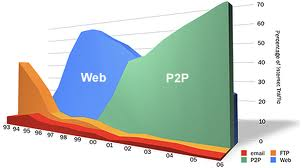
\includegraphics[width=5cm]{data/p2ptraffic.jpg}
\end{center}

However, New data from Arbor Networks shows that global P2P traffic is continuing to decline. 
Below there’s a graph posted by p2p-blog with the rate of decline, as compared with the overall Internet traffic between 2007 and 2009:
\begin{center}  
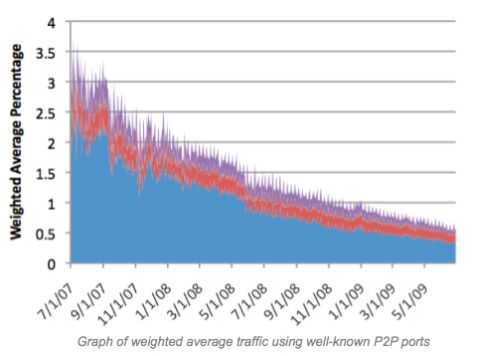
\includegraphics[width=5cm]{data/Arbor-Networks-graph-of-p2p-decline.jpg}
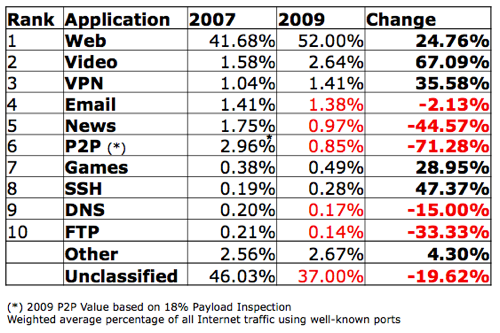
\includegraphics[width=5cm]{data/arbornetworks2-2.png}
\end{center}

There's a few interesting things to point out here: VPN traffic has been growing significantly at the same time as P2P traffic has been declining, which could at least in part be caused by P2P users signing up for VPN services to hide their activity.\cite{p2ptrafficdecline}

Obviously, this phenomemon indicates that on the suface P2P traffic declinies continusly and abundantly. On the other hand, the growing of VPN traffic enucleates that this kinds of shrink does not amount to vanish away but just migrate.
The root causes of this migratation is diversiform. 
However, we can deduce the most significant cause is the P2P applicaiton \emph{design objection} and \emph{vulnerable to attack}. 
So P2P users try to avoid these attacking and access blocked servers by using VPN, which seems to be an effective way to hide their actions. 
Unfortunately, most VPN services need extra fee to pay to these service providers before using it.
}

\subsection{Objections of Centralized P2P}
{
A typical Centralized P2P netorking is BitTorrent which implements multi-sources downloading and files distribution.
The basic fundamental of BitTorrent is the simultaneity of download and upload, which means when a user try to dowload resources from BT network, it also upload files or file segments to the others. So, the more users in the system , the faster will the files be downloaded. This incarnates the idea of 'tit-for-tat'.

When a user wants to share files or a directory, first of all, it has to generate a 'seed' file or 'metadata' file which contains the infomation about the shared files or directory and the URL of users.
And then upload the meta data to BT servers which are so called \emph{Tracker servers}.
Another user wants to download the shared file, it has to get to meta data from the Tracker servers, and then according to the infomation which is supported by the meta data to download the segments of shared files or directory from multipule resource nodes.
The follow chart illustrates the Architecture of BitTorrent:
\begin{center}
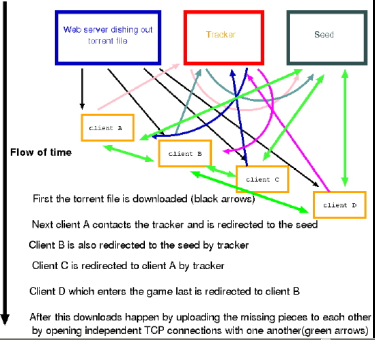
\includegraphics[width=8cm]{data/bittorrentprotocol.png}
\end{center}

From a structural point of view, BT belongs to centralized topology.
The Tracker servers are as a important part of the whole BT system, so the single point of failure performance failure should be inevitable. Moreover, BT does not support any search service, users have to login the BT published web server to find the files that he/she might be interested.

In this BT-liked centralized P2P networks, most noeds are connected with the centralized server or directory server which take the charge of indexing the context in all of the nodes. 
When request is sent, the centralized server will find all of the nodes which meet the qualifications of the request pre-sent. 
And then the file exchange will happen in the specified two nodes.

Taking one with another, the drawbacks of centralized P2P are as followed:
\begin{itemize}
\item Search calculation tasks are done by the centralized server, which may lead to a high requirements of server performance and bandwidth .
\item If the centralized server did not update in time, the result of the search task could not be accurate.
\item Due to the centralized server, the the single point of failure performance failure should be inevitable.
\item It is easy to cause "hot spots"phenomenon and copyright disputes.
\item Relatively weak ability to penetrate the firewall.
\end{itemize}

}

\subsection{Objections of semi-centralized P2P}
{
Typical semi-centralied P2P network applications are \emph{eMule\cite{eMuleProtocolSpecification} and skype\cite{SkypeTelephonyProtocol}}.
Different with centralized P2P network, semi-centralied P2P network has effectively avoided the design objections that are inevitable in centralized P2P network.
As to Skype, there are many \emph{Supernodes} to buildup the overlay network. This kinds of overly network contains two types of nodes --one is the supernodes mentioned above, the other is ordinary host machines.
The ordinary host is an running application which can initiate a session of communicaiton and can send message.
And the supernode is the ending point where the ordinary nodes login the Skype network.
Any common host machine which has been asigned the public address, and contains enough CPU,memory and network bandwidth can be selected as supernode. 
The ordinary nodes should communicate with the supernodes, register with the login server and login ,and then it can access the \emph{Skype} network.

In Skype, there is no centralized server except with login servers.
The store and transfer of login and logoff infomation , and the research request raised by users is in a distributed method. As a framework of P2P overlay network , there is few data stored in centralized servers in Skype.

The follow chart illustrates the \emph{Skype} network structure:
\begin{center}
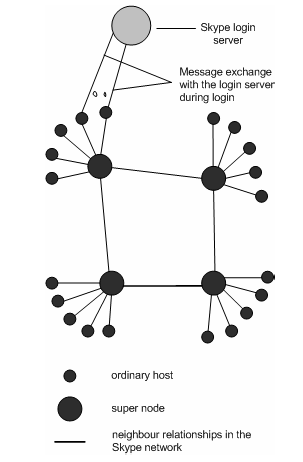
\includegraphics[width=4cm]{data/skypestructure.png}
\end{center}

Without a doubt, Skype, as a bussiness software has been reached great success in its own area --- VoIP.
The voice quality and the technique of codec is far better than other similar products.
Skype ocupied the large market share of P2P software.
However, P2P network does not provide existed solution for inevitable and potential security issues, Skype used private protocols and involved security issue, so the design and implementation were very complicated.
The management of supernodes is an onerous thing; the infomation of supernodes is stored in ordinary nodes for login and logout which is easily obtained and modified by hackers or somebody with intention, so it is more frail to suffer Sybil attack.

}

\section{Chanllenges Confronted}
{
It was because that we foucsed on the decentralized structured P2P network which was in order to avoid the design drawbacks that existed in other kinds of P2P networks, and considering with the VoD services , we should involve both the P2P overlay network and the VoD servicec based on the network we have constructed.

}
\subsection{Video File spliting ,publishing , recomposing and management}
{
  There should not be any video data centers to store and managethe video files which would send to different users to enjoy the VoD service in centralized structured P2P networks. That means we need to find an effective mechanism to handlethe actions on these video files.

Firstly, whether the video spliting is necessary or just we distribute the video files in a while block? We should consider the network service environment and anaylse the requirements which should also involve the VoD serice performance. 
In a large scaled network, a quite number of users request the same video at the same time; a great deal of connections will be established with the nodes which contain the resource files. Usually, the number of the resource nodes or seed nodes in the network is not quite many, that means less nodes will deliver the files to much more other nodes.
In this situation , the decentralized network will degrage to the semi-centralied network, these seed nodes will become the supernodes then. this is not what we expected.
As the mentioned above, we need to splite the video files into pieces and deliver the each piece to separate nodes.
Inspired from BT and eMule but not the same, we need to change the design so as to fix the request the VoD service.
And the \emph{granularity} of the spliting stream should be estimated.

Secondly, before spliting, the video stream may be encoded as many different formats, such as mp4, rmvb, wav, and so on.
So we should make the decision that whether we convert video stream from different formats to the controllable \emph{OGG}  format before delivering or just after gethering the pieces from the network and recomposing them then we convert the stream format.
Acutally, no matter when we convert the stream in the whole process, it is inevitable. The visible diffeerence is if we convert the stream after gethering data, the user impact is much more obvious. The client supported to user should pay much time to do converting and playing at the same time, which should influent the performance of VoD. However, if we just do it before delivering, the impact was just foucsed on the process of publishing.
And the efficiency we consumed in publishing will not impact user experience starkly.

Thirdly, what kind of swarming mechanism we should take. The mechanism will determine the attribute of \emph{KadPeer} project.
Usually, there are two kinds of mechanisms for data gethering -- push and pull. Both of the two are based on the Gossip algorithm. Much more effort and anaylse has been done in \cite{LargeScaleLiveMedia} and \cite{PushbasedSceduling}.

}

\subsection{Content Distribution and Search}
{
  As what we have assumed, there is no data center in the global internet, the publishing action is user spontaneous, so all of the data should be distributed in the whole system, which brings us chanllenges that it is hard to locate the chunks or segments which composed the total video files that user may request.
This part of phases depends on the mechanism we choose for swarming and diffusion.
And we also assumed the whole network is decentralized structured , so each peer will has a unique identifier. 
First connects the bootstrapping peers and selects one or several peers to construct logical links. 
Every peer maintains a group of logical neighbours and a routing table.
Peer selection is according to the routing table mentioned above.
This is also the spirit of \emph{DHT} and \emph{Overlay network}.
The key issue here is the data content distribution should match the logical routing mechanism for locating and searching.

Compared with the existed applications, just a few of them are focusing on the feature of user spontaneously publishing.
My purpose is to design and implement an easy accessing and high performancing \emph{VODFS-liked} system as an important component of the VoD application, which make peers faciliate to publishing their video data and to swarm video chunks from the other peers.

}

\subsection{Buffer / Cache}
{
As a basic function of \emph{VoD} , playback and random-index play are the most important features for \emph{VoD} applications.
To faciliate users with high quality and less response time, the application should have to decide upon the cache buffer size and cache.
}

\subsection{Stream Scheduler and metadata}
{
The scheduler keeps track of all the media content, which can be considered as a fraction of distribution and swarming mechanism.
Here, I prefer to explain the relationship between scheduler and metadata in my project.
My purpose is to design a effective method to maintain the scheduler according to the meta data which may affect the implementation of the VoD application.
An efficient and good quality matadata infrastructure for Video on demand can help in browsing and searching through the videos.
The chuncks of a specific video may attain to the peer disorderly, there should be a prepared Buffer-Map table which defines all of the chuncks splited from the whole video bulk.
The metadata could contain the Buffer-Map which is used to index the chuncks of a video and provide an absolute timing sequence of playing process which could be easily handled by the video exhibition engine.
Moreover, the metadata could be published as an item of program list which could be searched by the users who are interested in the keywords that the matadata contained.

Also there is another way to mantian the chunck order or time sequence without metadata.
There are field selections in \emph{OGG stream} with the name of \emph{bitstream serial number} and \emph{page sequence number} which define the logical bitstream identify and the page sequence. 
The sequence number increasing on each logical bitstream separetely can identify page page loss by the decoder.
However, in this situation, if we implement the scheduler just depending on the sequence number provided by the bitstream itself, the function of search should be weaken and raise the difficulty standard of decoder, especially when the bitstream contains multipule logical streams or stream groups.
This is not what we expected.
}

\subsection{GUI and Video exhibition}
{
This is the most user impact part of the \emph{VoD} application. It provides the GUI client to the users or customers and also provides control pane for item selecting, jumping forwards ,jumping backwards and other actions.
I did not pay much effort on the design of user interface, because this is not the most important thing for the current phase. It could be the future task of my project.
However, Video exhibition should be the most urgent issue of the system which determines the performance of the VoD simulation.

As for the video exhibition feature, it should contain three components --  video , audio and caption.
The key chanllenge of this issue should be the integration of the three components.
Currently, there are much many media player on the market including the opensource and non-opensource.
My project is \emph{OGG} bitstream based and current the resources of common media players are stored in local or ordered stream from the internet such as \emph{RTP} and \emph{RTSP}, that means I have to implement a codec which can distinguish the three kinds of streams with disodered chuncks and also can exhibit them to the users.
}

\section{Summary}
{
In this chapter, I have illustrated the decline of P2P traffic, the core reason is that the traffic has been hiden behind the VPN service.
I have analysed the drawbacks of centralized and semi-centralied P2P network which is inevitable because of the design.
And also I provide the chanllenges that I have confronted in the design and implementation.

}

\chapter{Kademlia Network Customization and Analysis}
\label{cha:cha2}
{
Kademlia is a communication protocol for P2P overlay networks. 
It is one of many versions of a DHT, which is designed by Petar Maymounkov and David Mazières.
A Kademlia network is characterized by three constants, which were called \emph{alpha, B, and k}.
\emph{alpha} is a small number representing the degree of parallelism on network calls, usually 3.
\emph{B} is the length of keys used to identify nodes and store and retrieve data.
\emph{k} is the the number which indicates the max size of a k-bucket that contains the contacts.
Simply to say, the DHT of kademlia is different with that of Chord, CAN, Pastry and other algorithms, because Kad uses a special \emph{XOR} metric as the base of the distance calculation, which establishs an absolutely new DHT toplogy structure that advances the speed of route quering.

Kademlia itself doese not specify how to do file sharing or other network services, but defines the routing policy of communication, and four RPCs protocol functions to maintian the system which are PING, STORE,FIND\_NODE and FIND\_VALUE.
This chapter will illustrate the work mechanism of Kademlia and customization on searching and publishing which enhances the performance of KadPeer services.

}
\section{Distributed Database -- DHT}
{
P2P system usually holds a Distributed DB to publish and search entries.
Also \emph{Kademlia} maintains a distributed database, which is a Distributed method to store data. 
In the case of the needless of server, each client takes a small scope of routing table, and also takes the role of storing a fraction of data, so as to implent indexing and stroring of the whole DHT network.
The follow chart illustrates the framework of \emph{DHT}:
\begin{center}
  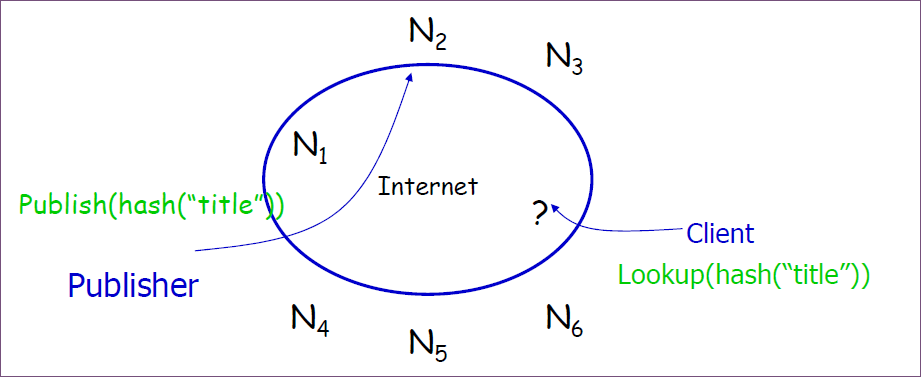
\includegraphics[width=10cm]{data/DHT.png}
\end{center}

A typical KAD DHT network may contain two dictionaries -- ``keyword dictionary'' and ``file index dictionary''.
The keyword dictionary uses the provided keyword to query the responded file name and file information. 
The key equals to the 160-bit \emph{SHA-1} hash output of the keyword; and the responded value of the key will be a list, in which lists all of the responded information of the keyword related to the file name.
Usually, these information can be presented as a triple element (file name, file length, SHA-1 value). 
The file index dictionary is used to query the file owner according to the provided file information. 
The key equals to the \emph{SHA-1} checksum of the file to be downloaded. This is because, as the aspect of statistic, the 160-bit \emph{SHA-1} checksum can ascertain a data file with specific content.
And the value to the key will be be a list as well, which contains the network information of these ndoes which might have the file.
The item of the list can be present as a triple element(IP,Port, Owner ID), by which the P2P application can query the node who has the file copy with same \emph{SHA-1} value.

}


\section{Sketch of Kademlia}
{
\emph{Kademlia} (KaD in short) is a technology of Distributed Hash Table (DHT), and the main issue of which wants to solve was information storing and indexing with distributed network-wide approach to the application layer.
In the global KaD network, all of the information were stored in the form of \textless key,value\textgreater  hash entry.
And all of the hash entry were distributed to separated nodes, and the network-wide emerged to a huge hash table. 
We can image the huge hash table to be a dictionary, that means if we get the key of index information, we can use \emph{Kademlia} protocol to locate the responded value without knowing which node the value was stored accurately.
\emph{Kademlia} takes the key role of file information indexing.
The follow chart illustrates the architecture of Kademlia protocol.
\begin{center}
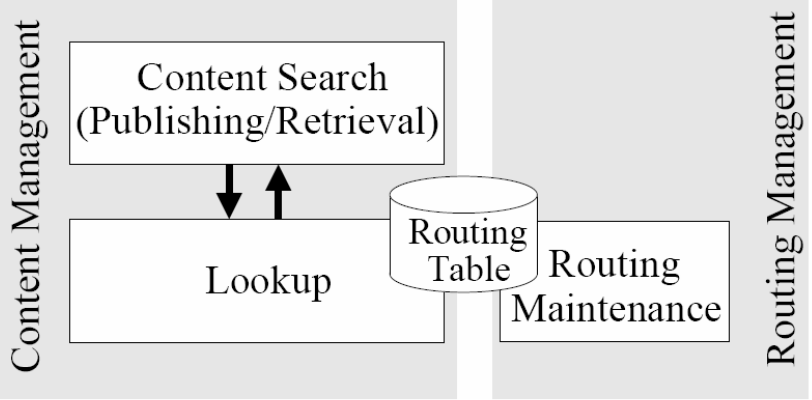
\includegraphics[width=8cm]{data/kadarchitecture.png}
\end{center}
}

\section{Components Customization of Kademlia Service}
\subsection{Routing}
\subsubsection{XOR Metric}
{
Each node in \emph{KaD} has a unique ID as identifier. 
As to the formulation of the ID, different application might have different implementation, an ordinary method was to select a unique value and do \emph{SHA-1} calculate, the unique value could be the IP of the user, or just be generated randomly.
In \emph{KadPeer} project we assume that the ID is with 160-bit length, compaired with 128-bit of the original kademlia specification.
That was because I define the length of ID is 160-bit which is the same with that of the output of \emph{SHA-1} calculation.
The distance between two nodes depends on a \emph{XOR} metric of their nodes IDs which identified the specify node.

Let node J = j$_{m}$...j$_{30}$..j$_{2}$j$_{1}$ and node K = k$_{m}$...k$_{30}$...k$_{2}$k$_{1}$, so the distance between node J and K can be calcualted as :
\begin{equation}
d(j,k) = \sum_{i=1}^{m}{
  \left\vert 
j_{i} -k_{i}
  \right\vert * 2^{i}
}
\end{equation}

we can also easily derive that the closest ID of a specific node is unique.
\begin{equation}
%\begin{align}
d(j,k) = d( j^{'},k) \Leftarrow\Rightarrow j = j^{'}
\end{equation}
\begin{equation}
d(j,k) >= 0
\end{equation}
\begin{equation}
d(j,k) = d(k,j)
\end{equation}
\begin{equation}
d(i,j) + d(j,k) >= d(i,k)
\end{equation}
\begin{equation}
d(d(i,j),d(j,k)) = d(i,k)
\end{equation}

The advantages of this \emph{XOR} metric are obvious. 
Firstly, it was easy to calculate.
Secondly, it was symmetrical which means that if node j is close to node i then node i is also close to j.
It will be useful to learn new contacts (routing table entries) just by receiving communication requests from other nodes.
}

\subsubsection{K-Bucket}
{
The routing table of Kademlia is composed by these lists which are so called k-bucket.
This is allied to \emph{Tapestry} algorithm whoes routing table is constructed similarly with that of kademlia.
Each node will store some information of these contacts with which the distance between them is in the scope [ 2$^{i-1}$,2$^{i}$) ( 0 \textless= i \textless= 160).
In the other implementation of kademlia , these information of contacts that stored in a node is composed by list of Node ID, IP and UDP port.
However in \emph{KadPeer} , it was much more complex, because I added the function of tunnel through NAT and firewalls based on the \emph{UDT} library.
I reserved the fileds of rendezvous ip and port for additional usage.
Each list of the information is so-called \emph{K-Bucket}, and the contacts in the bucket is sorted by the last visit time.
The last-recently contact is in the list head, and the most-recently is in the head tail.
Each bucket has its max size of contacts which is characterized by variable \emph{K}.
Usually, K is an even number which is used to balance the system performance and the network load.
The chart below illustrates the structure of a K-Bucket.
\begin{center}
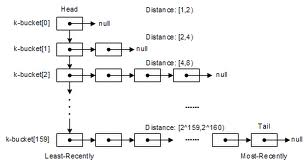
\includegraphics[width=8cm]{data/kbucket.jpg}
\end{center}

When variable ``i'' is very small, the K-Bucket will be empty; while the variable increasing, the items in the bucket will exceed K.
It is because the growth of the discance that the K-Bucket covered is exponential, that means a node will know more the closer neighbors and less farther ones which ensures the convergence of the information query process.
That is to say, every node knows well of its neighbors and as the distance growth the degree will decline.
As the interval is divided by exponentially, so the complexity of key looking up of a N nodes kad network is log(N).
This feature is simliar with that of \emph{Chord} fingertable of interval spiliting.
When a node i receives a RPC message , the sender node contact info of j in i node's k-bucket will be updated.
The steps are as followed:
\begin{enumerate}\itemsep1pt
\item Calculate the distance between iteself and the sender node : d(i,j).
\item Select responded K-Bucket to do update according to the calculated distance d.
\item If contact of j is on the selected bucket, then move the contact to end of the bucket.
\item If contact of j is not on the selected bucket
\begin{enumerate}%[I]%
\item If the size of the selected bucket is smaller than k, then add the contact information of node j to the end of the bucket.
\item If the size of the selected bucket is greater than k, then select the head contact z in the bucket to do Ping RPC.
\begin{enumerate}%[(a)]%
\item If the z node doese not send the response message, then delete the contact of z and add contact of j to the end of the bucket.
\item If the z node sends the response message, the move contack of z to the end of the bucket and drop j.
\end{enumerate}
\end{enumerate}
\end{enumerate}

The mechanism of bucket update method implements the strategy of updating last-see node, unless the on line nodes have never been removed from the bucket.
That is to say, the longer the node on the line, the more it will be leaved on the K-Bucket.
With this mechanism, KaD can obviously improve the online rate of the contacts in the bucket.
This will bring up greate advantages on the stabilty of kad network and decline of maintenance cost.
On the other hand, this mechanism can defend \emph{DDos} attacking, as only when the old nodes are out of ervice, these new nodes can be joined into the k-bucket, which avoids the flooding of the routing information caused by joining of the new peers.
In order to prevent the K-Bucket from getting old, the KaD will select some node from the k-bucket it contains to do RPC\_PING during the interval that there is no k-bucked updated.
The mentioned updateing mechanism of KaD moderates the bottleneck of the traffic, all of the nodes will not do the updating operation at the same time.
At the same time, KaD can respond the nodes which are out of service rapidly.
}

\subsubsection{Routing Table Evolution}
{
When Node u wants to joion the KaD network, it should communicate with an existed node w.
First of all, u adds contact of w to its own K-Bucket, then send a RPC\_FIND\_NODE.
After that, u will update its K-Bucket according to the information that has gethered.
By quering the neighbors from far to near by steps, node finished the construction of the empty routing table, and publish the contact of its own to the neighbors.
In KaD, the routing table of each node is present as a binary tree, and the leaf can be considered as a K-Bucket.
We take node as an example, the process of routing table construction is as followed:
\begin{enumerate}
\item At first, routing table in node u is a simple K-Bucket, which covered 160-bit ID space.
\item When u learned some new node information, it will try to add these information to the responded K-Buckets:
\begin{enumerate}
\item If the K-Bucket is not full, then the new node will inject into the K-Bucket.
\item If the K-Bucket is full:
\begin{enumerate}
\item If the current bucket scope covered the ID of node u, then the current bucket would be splited as two bucket with the same size. And reassgin the contacts in each new bucket according to the prefix value.
\item If the current bucket scope does not cover the ID of node u, then the contact of u will be dropped.
\item Repeat the process listed above, and at last the routing table will be constructed which contains much contacts that are near by and less contacts that are far away.
\end{enumerate}
\end{enumerate}
\end{enumerate}
The chart below illustrates the process of K-Bucket splitting.
\begin{center}
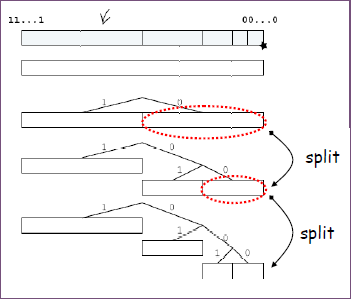
\includegraphics[width=8cm]{data/TableSplit.png}
\end{center}

}

\subsection{Searching}

\subsubsection{Iterative Quering}
{
There are two types of data quering methods. 
First is iterative quering , the second is Recursive quering.
KaD uses iterative routing for quering.
In the process of iterative quering, the source send look-up request the next hop and wait for its reply, and then according the content of the reply to query the next hop till the iteration depths reached the max value or the source has got the reqeusted data.
However ,in the process of Recursion quering, the source send look-up request the next hop but do not wait for the reply of that hop.
The second hop queries its own database to check if it has the data that the source requested.
If the hop contains the data that reqeuested, it will send the response to the source or query the next hop depending on the routing table it has till the recursion depth reached the max value.
The follow chart illustrates the core differences between iterative quering and recursive quering.
\begin{center}
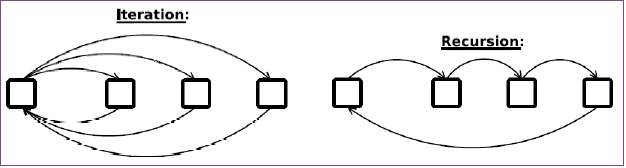
\includegraphics[width=8cm]{data/IterativeLookup.png}
\end{center}

Considering with the process of iterative quering, the source is responsible for the whole process, and at each step, source send requests and wait for the reply,
so the advantages of iterative quering are much easier to observe:
Firstly, Lookup messages cannot be lost due to the departure of an intermediate peer holding the lookup request.
Secondly, Iterative routing is easier to debug since information at each step is reported back to source.
}



\subsubsection{Parallel Look-Up}
{
In Kademlia algorithm, in ordor to reduce the problem of hitting stale contacts and improves lookup performance, it takes parallel mechanism to do data look up, although this will inevitably brings up the traffic of quering process.
Source simultaneously issues multiple lookup requests to different peers and continues the lookup process based on the information obtained from all requests.

The follow chart illustrates the process of parallel look-up.
\begin{center}
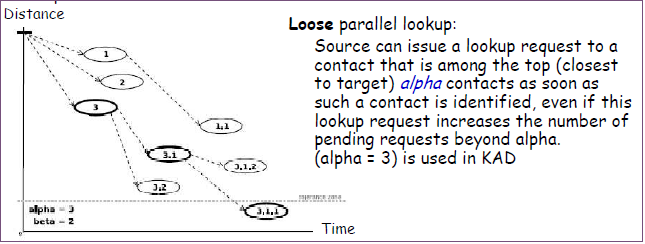
\includegraphics[width=15cm]{data/ParallelLookup.png}
\end{center}

%Source can issue a lookup request to a contact that is among the top (closest to target) alpha contacts as soon as such a contact is identified, even if this lookup request increases the number of pending requests beyond alpha. (alpha = 3) is used in KAD.
}

\subsubsection{Kad Node Status}
{
In \emph{Kademlia} network, all of the nodes can be considered as a leaf of a binary tree, and the location of a node was decided by the shortest prefix of the ID.

For any node can separate the binary tree into series of continuous, non-self-contained subtrees.
The top level subtree was composed of the whole tree excludes the subree of its own, and the next layer subtree was composed of the rest half subtree;and so forth, till the whole tree was separated. The next chart illustrates how to separate a tree by node ``0011''.
\begin{center}
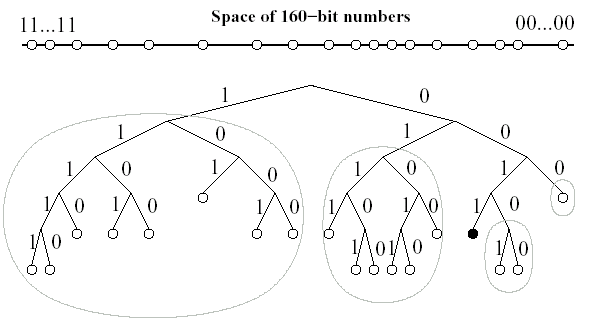
\includegraphics[width=10cm]{data/kadbintree.png}
\end{center}

The parts which were contained by dotted line were respective subtrees. the prefix from top to the bottom were `1','01' ,'000' ,'0010'.
\emph{KaD} protocol makes sure that each node knows at least one node of the subtrees, as long as these subtrees are not null.
In this context, each node can find the other nodes by the unique ID.
The process of routing was obtained through the efforts of the distance of \emph{XOR}.
The chart below illustrates the way that how does node ``0011'' find the node ``1110'' by continuously quering.
The node ``0011'' accesses closer to the ultimate target node convergently by progressive learning and inquiry among the bottom of the sub-trees.
Should be noted that, the only node ``101'' was known by node ``0011'' . 
\begin{center}
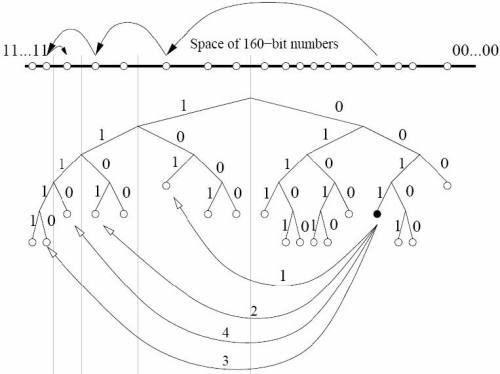
\includegraphics[width=8cm]{data/kademlialookup.jpg}
\end{center}
Should be noted that, the only node ``101'' was known by node ``0011'' 
}

\subsubsection{Optional Choking}
{
In Kademlia, there is no definition of the policy on contact choosing while the RPC FIND\_VALUE reply of quering contains multiple contacts.
A FIND\_VALUE RPC includes a B=160-bit key. If a corresponding value is present on the recipient, the associated data is returned. Otherwise the RPC is equivalent to a FIND\_NODE and a set of k triples is returned.
However, In the project of \emph{KadPeer}, I defined a policy on contacts choking based on a third party project with the name of \emph{GeoIP} which may improve the performance of P2P network services.

GeoIP is the proprietary technology that drives MaxMind's IP geolocation data and services. GeoIP provides businesses with a non-invasive way to determine geographical and other information about their Internet visitors in real-time. 
When a person visits the website, GeoIP can determine which country, region, city, postal code, and area code the visitor is coming from. 
Furthermore, GeoIP can provide information such as longitude/latitude, connection speed, ISP, company name, domain name, and whether the IP address is an anonymous proxy or satellite provider.

As the feature provided by \emph{GeoIP}, in the reply of RPC quering, the \emph{KadPeer} will get the reail time information of the contacts by calling the GeoIP API.
It will sort the contacts by the connection speed and choose these contacts which are with high connection speed for data downloading and uploading.

}

\subsubsection{Node Searching and Locating}
{
The supreme feature of Kademlia algorithm is the mechanism of quickly node searching, and the steerable quering process by changing the key parameters such as \emph{alpha} and \emph{k}.
We assume node x want to find the node whos ID is y,  kad will do as followed process to locate node y.
\begin{enumerate}
\item calcute the distance between x and y, d = d(x,y).
\item Select $\alpha$ nodes from the [log(d)$_{th}$] K-bucket of node x, and send FIND\_NODE RPC to the $\alpha$ nodes. If the the number of contacts in the K-BUCKET is less than $\alpha$, then select the enough contacts from the buckets which are closer to d.
\item As to the contacts on the reply, if the current node is y, then send the reply to the source that it is the closest node to y. Otherwise, cacluate the distance to y, and select $\alpha$ contacts from responded K-BUCKET to send to x.
\item x will send FIND\_NODE RPC to the received contacts in the reply, and redo the process till that there is node which replys the nearest ID to y in each branch. These nodes which are not quickly responded will exclude from the candidate list till they send the reply.
\item Through the operation listed above, node x will get k contacts which are closer to node y. 
Because node y might not be in the internet, we say the closer here.  $\alpha$ is the parameter which controls the parallel degree. When $\alpha$ = 1 , the searching process will be simliar with \emph{Chord} quering hops.
\end{enumerate}

Because source can get information from the bucket which is closer to destination during the query each time, this mechanism ensures that the distance to the target will be halved or at least decline one bit.
So, the efficiency of Kademlia algorithm will be log(N), and N indicates the number of nodes in the kad network.
When node x wants to search \textless key,value\textgreater, the operation is similar to search a node.
Node x will choose k contacts which are closer to key, and send FIND\_VALUE RPC to them. Then redo the process to the contacts which are contained in the replys.
When RPC FIND\_VALUE succeed, the \textless key,value\textgreater will be stored in the node which is the closest to key, so as that it will enhance the performance of quering next time.
By this way, the scope of hot \textless key,value\textgreater will be expanded,which makes the acknowledgement of whole system become more shorter.
}

\subsection{Publishing}
{
In Kademlia specification, there is no definition of how and where to publish data that users might be interested. But, it defines the interval to republish and expire which ensures that the data in the system is fresh.
However, publish process is another important performance indicator of P2P system.
}

\subsubsection{Where to Publish}
{
Where to publish a given key kID?
Unfortunately, the original \emph{Kademlia} does not define the method to the publish.
I have referred the way that how does \emph{Chard} and \emph{Emue} to publish the given data.
In \emph{Chord}, the given data will be stored in the first node with which the ID is larger than the kID.
However, in the implementation of \emph{emue}, there is a concept with the name of zone, in which the first 8 bits of the nodes are the same.
8 bits is the 1/256 of the entire key space( The key space of emue is 128 B), which contains several thousand of peers.  
In my project \emph{KadPeer}, I also followed the conception of zone.
However, I define the zone in which the first 16 bit of the nodes are the same, as the key space of kadpeer is 160-bit.
And when publishing, 16 nodes which are in the same zone with the KID are choosen for uploading the data.
That means 16 copies of publishing data will exist in the network, and this number will grow depending on how hot this data is as the time elapsing.
That is because while searching the hot key, when the source finds the key, it will send RPC STORE\_VALUE to the closest contact in its bucket to store the hot key and value pair.

However, how to find these nodes in a 16-bit zone?
To get the 16-bit zone, the source will send RPC FIND\_NODE with the parameter KID, this will obtain an ordered (by closeness) list of nodes that are up the KID.
After that, the source will send RPC PUBLISH\_REQUEST to the closer candidate nodes.
In each nodes, there will be a specify data store with multiple index and a mark field, which indicates the wether the data is published or just a common data.
In kadpeer, in order to obtain a high performance of data storing and searching in a node, I did not use  database sucha as mysql as the data store.
I implemented a data structure which can reorder the content with two indexes.
Any data published in the network will be stored in the computer memory, which ensures that the data will keep fresh cooperation with the republish policy of the kademlia algorithm.

\subsubsection{How to Publish}
Another important issue is how to publish the data.
Compared with the other P2P application, in kadpeer network there is only two kinds of data.
One is metadata of a media stream, the other one is stream data.
While publishing, the splitting engine will split the OGG stream data to pieces, and meanwhile the metadata will be generated, which contains the file name and important OGG stream information.
So, when we publish a media stream, we need to publish two components of an entry.
I defined a two-level publishing steps here.
Level 1 indicates the hash value of metadata information.
Level 2 indicates the hash media content data which has been splitted into pieces by the OGG codec engine.

We assume that a client wants to share a media file with the name of ``kademlia project''.
\begin{center}
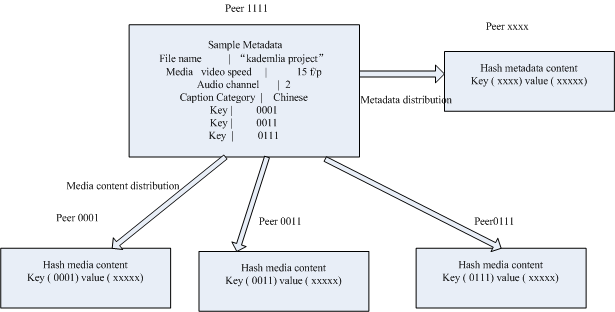
\includegraphics[width=15cm]{data/Distribution.png}
\end{center}
The OGG codec firstly parse the media file, and generate the metadata according to the content of the media, which contains the hash value of each media stream pieces.
%The ``kademlia project'' was divided in to several pieces, which content hash value was ``0011'' 
Each hash value will be the KID which covered the global kadpeer ID space.
The publisher will then distribute each hash key and value pair of the media to the 16-bit zone which covered with the key ID.
It is because that the metadata is the only identifier of a specify stream.
We need to publish it to the network so as to the other peer can find it as well.

%\begin{center}
%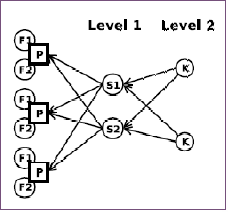
\includegraphics[width=5cm]{data/TwoLevel.png}
%\end{center}

}

\section{Summary}
{
%This chapter, I have illustrated the way that the \emph{Kademlia} network worked, and also interpreted the customization on the algorithm.
The latest work of P2P is incarnateed on the decentralised structured network toplogy basd on DHT.
The essence of DHT is a huge hash table which is maintained by a profusion of nodes in union.
The DHT is splitted into pieces, and each node will maintain a chunck of table which belongs to it.
The nodes of DHT is dynamic and also is generous,so decentralised-structured and self-ruled are the importand target of design.
An object or a keyword can be hashed to a 128 or 160 bit space by calculating the hash function.

DHT liked structure is self-adapting for node join and leave, and with good performance, expandability, vigorousness, and the ablity of self-organization.
It is because that the overlay network adapt to confirmative structure, the DHT can support accurate discovery.
As soon the node is on the network as it could be found.
This chapter will illustrate the work mechanism of Kademlia and customization, which provides network modes for VoD on demond system.

}


\chapter{Design and Implementation of KadPeer}
\label{chap3}
{
The architecture design was done according to the effort paied to the study of the issues that addressed.
A lot of time has been spent on the project was used to study a possible solution of \emph{OGG} file spliting and merging.
I obtained the simplest possible method to the spliting policy using the characteristics of containers and codecs of \emph{OGG}.

To obtain the P2P integration the quality streams will be encapsulated into a metadata file which was inspired from the design of BitTorrent.
The metadata will contain the infomation of the ordinary stream and also extra track infomation which is used for initiating the decoder.
However, my P2P related design does not depend on the BitTorrent but \emph{kademlia} ,the decentralized structure infrastructure.

At first sight it was clear that the only way to go was to exploit the possibility of assigning media chuncks to different peers of a metadata to be able to download the part by not lossing pages of stream. As we are going to see later this feature is the heart of scheduler controller which enable to downlaod the chuncks with correct order.
}

\section{Overall Design Precept Description}
{

The \emph{KadPeer} aims at the \emph{VoD} services which provides high performance of video playing includes audio and captions as well, and also allows users search the video content he/she interested.
And the features list as followed:
\begin{itemize}
\item Login and logout the network system. (basic, but GUI interface is optional and it will be future task)
\item Interface to publish the media data. (basic)
\item Search the media resource that the users might be interested.(basic)
\item List up the known resource in the internet.(basic)
\item Play the Video that user select from the known resource list or search result.(basic)
\item Jump forwards and jump backwards of video on playing arbitrarily.(basic)
\item Download the video resource directly from the search result.(optional)
\item Tranfer data through NAT or firewalls.(optional)
\end{itemize}

In allusion to the features list above, I gave out the related design ideas and the resolvent.
The chart below illustrates the global structure of \emph{KadPeer}.
\begin{center}
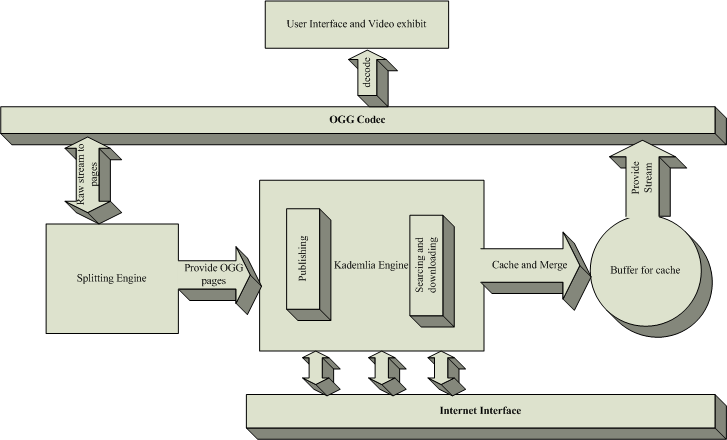
\includegraphics[width=15cm]{data/KadPeerStructure.png}
\end{center}
As we can see from the above chart, there are two important engines in KadPeer.
One is kademlia related which handles the backend video distributed and swarming, the other is video data operation related which handles video content parsing and provides basic infomation for OGG codec to do video splitting.

To implement \emph{KadPeer}, I have anaylsed and take the usage of more than 10 librarys which covered the important functions of the client, such as thrift, libogg, libtheora, libvorbis,libkate, and oggplayer.
I will select some of the important librarys to illustrate how these third part librarys worked in kadpeer later.
}

\subsection{Important Third Part Libs and the Integration}
\subsubsection{Thrift}
{
Thrift is a software library and set of code-generation tools developed at Facebook to expedite development and implementation of efficient and scalable backend services. 
Its primary goal is to enable efficient and reliable communication across programming languages by abstracting the portions of each language that tend to require the most customization into a common library that is implemented in each language.

Specifically, Thrift allows developers to define datatypes and service interfaces in a single language-neutral file and generate all the necessary code to build RPC clients and servers.

The base types supported by Thrift are:
\begin{itemize}
\item \texttt{bool} A boolean value, true or false
\item \texttt{byte} A signed byte
\item \texttt{i16} A 16-bit signed integer
\item \texttt{i32} A 32-bit signed integer
\item \texttt{i64} A 64-bit signed integer
\item \texttt{double} A 64-bit floating point number
\item \texttt{string} An encoding-agnostic text or binary string
\item \texttt{binary} A byte array representation for blobs
\end{itemize}
Also, Thrift defines a common object to be used across languages. 
A struct is essentially equivalent to a class in object oriented programming languages. 
A struct has a set of strongly typed fields, each with a unique name identifier. 
The basic syntax for defining a Thrift struct looks very similar to a C struct definition. 
%Fields may be annotated with an integer field identifier (unique to the scope of that struct) and optional default values.

In KadPeer, for the kademlia engine implementation, RPC related functions are based on the Thrift library.
Additional structs of thrift has been defined in kadpeer such as ``ContactInfo'',''signed\_kadvalue'' and ``kademila messages'', in which the exchange data are contained during the communication process.

%Thrift reduces the effort that I should pay for on the 
}

\subsubsection{libogg,liboggz,libtheroa,libvorbis,libkate}
{
%The librarys listed above are \emph{OGG} container.
Oggz provides a simple programming interface for reading and writing Ogg files and streams. Ogg is an interleaving data container developed by Monty at \emph{Xiph.Org}, originally to support the Ogg Vorbis audio format.
Support is built-in for parsing the headers of and seeking to time positions in Ogg Dirac, FLAC, Speex, Theora and Vorbis. 
Oggz is also compatible with Annodex streams, and supports seeking on all tracks described in an Ogg Skeleton track.

Theora is a general purpose, lossy video codec. It is based on the VP3 video
codec produced by On2 Technologies (http://www.on2.com/). 
On2 made an irrevocable, royalty-free license grant for any patent claims it might have over the software and any derivatives. 
Theora contains a superset of the features that were available in the original
VP3 codec. Content encoded with VP3.1 can be losslessly transcoded into the
Theora format.\cite{THEORA}

The Vorbis audio CODEC provides a channel coupling mechanisms designed to reduce effective bitrate by both eliminating interchannel redundancy and eliminating stereo image information labeled inaudible or undesirable according to spatial psychoacoustic models.
In encoder release beta 4 and earlier, Vorbis supported multiple channel encoding, but the channels were encoded entirely separately with no cross-analysis or redundancy elimination between channels. This multichannel strategy is very similar to the mp3's dual stereo mode and Vorbis uses the same name for its analogous uncoupled multichannel modes.\cite{VORBIS} 

Kate is an overlay codec, originally designed for karaoke and text, that can be multiplixed in Ogg. Text and images can be carried by a Kate stream, and animated. Most of the time, this would be multiplexed with audio/video to carry subtitles, song lyrics (with or without karaoke data), etc, but doesn't have to be.
Series of curves (splines, segments, etc) may be attached to various properties (text position, font size, etc) to create animated overlays. This allows scrolling or fading text to be defined. This can even be used to draw arbitrary shapes, so hand drawing can also be represented by a Kate stream.\cite{KATE}
}

\subsubsection{liboggplay}
{
\begin{center}
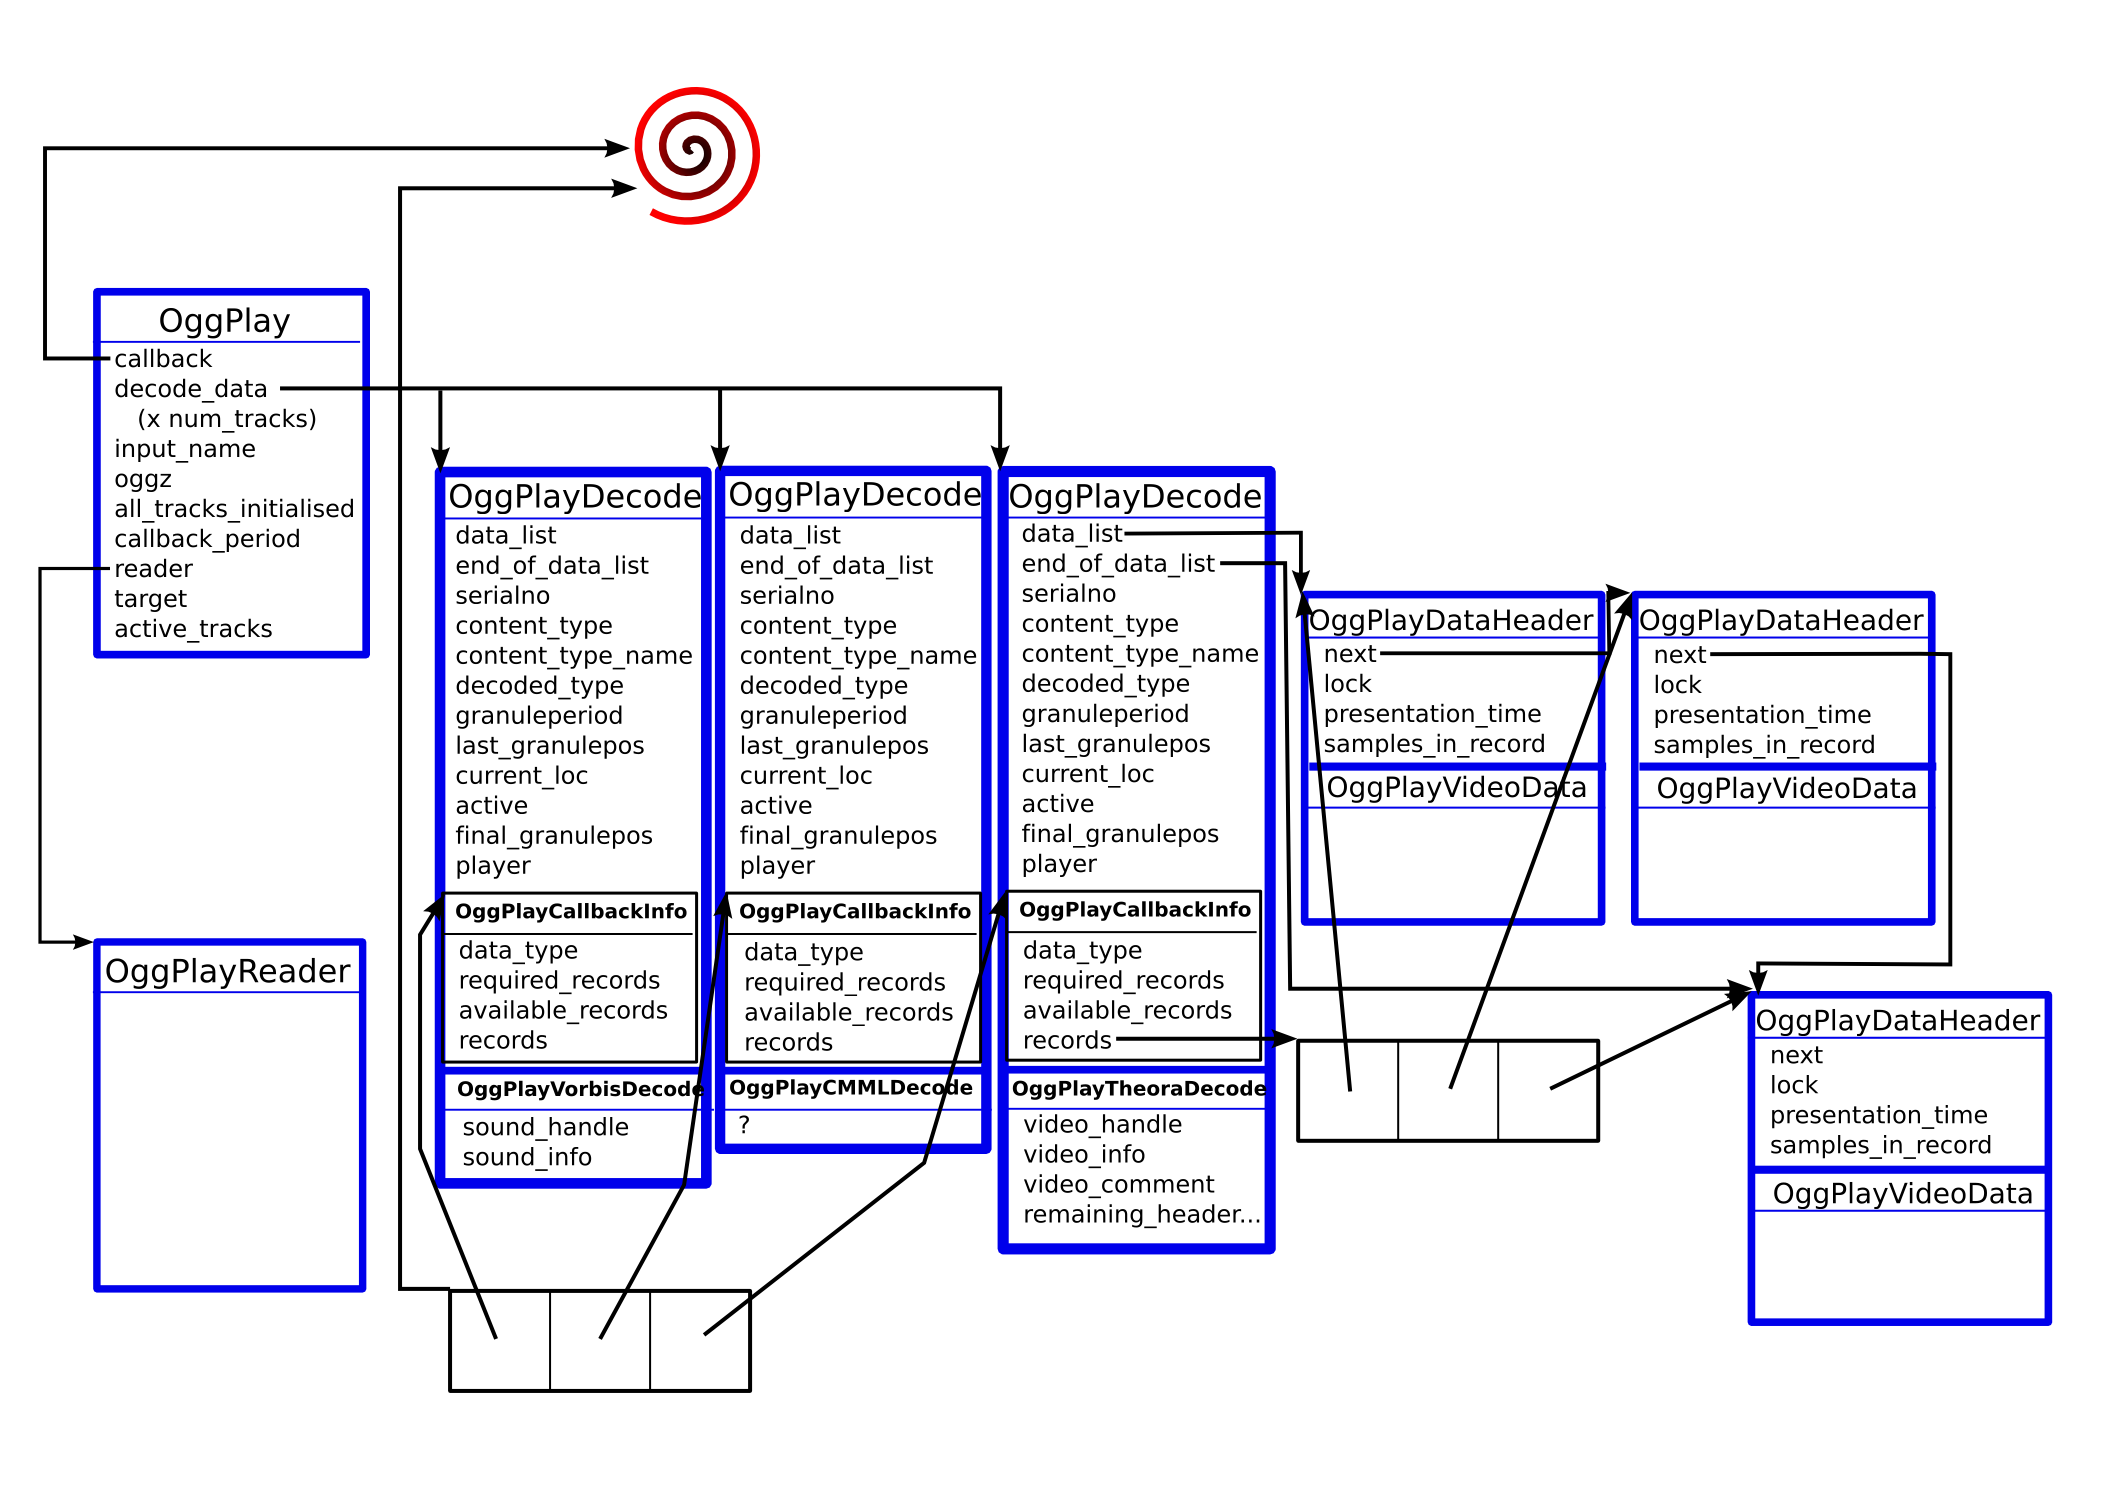
\includegraphics[width=15cm]{data/liboggplay_data_layout.png}
\end{center}
}

\subsection{Meatadata Format}
{
The problem of how to produce a metadata infomation according to the specify video stream was the first to be addressed.
Because of its big importance in the project. it has been considered from various points of view.

Let us review the torrent mechanism used in BitTorrent liked system. 
Torrent file is the most important part of the whole BT system, which includes the infomation of Tracker server and the the segments to download. 
We can consider the torrent file is the carrier of BitTorrent protocol. When using the BT to download a related file, you have to get the torrent file first.
Torrent file contains the basic infomation of the file to download, such as file name, file size, and location infomation of the file publisher server.
So, the BitTorrent client can search the server according to the infomation that torrent file provided.
At the end, an extra \emph{SHA1} checksum to ensure the integrality and validity of the segment.

what to be highlighted is the codec format of torrent file which was so-called "Bencode".
“Bencode" infomation contains string, dictionary and nestification of list.

The "Bencode" data structures are as followed:

%\begin{center}
\begin{tabular}{|l|c|l|}\toprule
Types      &  Express Mode                           & Sample  \\ \midrule
string     &  \textless length\textgreater :context  & 4:spam \\ \hline
Integer    &  \textless i\textgreater integer\textless e\textgreater          & i3e means decimal 3 \\
           &                                         & i-3e means decimal -3 \\ \hline
List       &  \textless i\textgreater Bencode Value\textless e\textgreater & l4:spam4:eggse \\
           &                                          &        means \\
          &                                            & ['spam','eggs'] \\ \hline  
Dictionary & \textless d\textgreater \textless Bencode String\textgreater \textless Bencode element\textgreater \textless e\textgreater &d3:cow3:moo4:spam4:eggse \\
        &                                       &means \\
           &                                         &   {'cow':'moo','spam':'eggs'}\\
\bottomrule
\end{tabular}
%\end{center}

A torrent file is a bencoded dictionary with the following keys:
\begin{itemize}
\item announce - the URL of the tracker
\item info - this maps to a dictionary whose keys are dependent on whether one or more files are being shared:
\begin{itemize}
\item name - suggested file/directory name where the file(s) is/are to be saved
\item piece length - number of bytes per piece. This is commonly 2$^{18}$ = 256KiB = 262144B.
\item pieces - concatenation of each piece's SHA-1 hash. As SHA-1 returns a 160-bit hash, pieces will be a string whose length is a multiple of 160-bits.
\end{itemize}
\end{itemize}

% And exactly one of length (corresponds to when only one file is being shared) or files (corresponds to when multiple files are being shared):
% \begin{itemize}
% \item length - size of the file (in bytes)
% \item files - a list of dictionaries (each dictionary corresponds to a file) with the following keys:
% \item path - a list of strings corresponding to subdirectory names, the last of which is the actual file name
% \item length - size of the file (in bytes)
% \end{itemize}
%All strings must be UTF-8 encoded.

As I have introduced the \emph{OGG format} in the begining of my thesis. 
Ogg file has different attributes compared with the other format files, so we can mux the design of BitTorrent to create new format of metadata infomation which can be used efficiently to manage the resource in the DHT environment.

However, I did not follow the ``Bencode'' format completely, great changes were committed to the design of metadata format.
\begin{enumerate}
\item Athough the ``bencode'' has been an easy way for encoding and parsing the content of a torrent file, I did not continue to use ``becode''. 
It was because I intended to combine more complex data format in the metadata info. And moreover, this new kinds of format should be more convenient to  transfer to string, we need to deliver the string on the internet arbitrarily. 
I take up \emph{XML} -- the structured language to mantian the metadata, which has been implemented by many opensource developers.
The most famous project which implements the \emph{XML} with C plus plus programming language is \emph{tinyxml} on sourceforge\cite{tinyxml}. 
The \emph{Tinyxml} has provided simple and convenient APIs to make it easily integrating into other programs, especially this XML parser is lightweight, stable and constructed with STL( when compiling , you should add special definitions to compile options to enbale STL.)which makes this integration more compact, because the \emph{KadPeer} is constructed with pure C++ in \emph{Linux } platform.
%TinyXML is a simple, small, C++ XML parser that can be easily integrating into other programs.
\item The elements to record the video file in metadata which users published or shared on the internet were changed compaired with the torrent components. 
I add additional infomation to the metadata such as track numbers among the \emph{Theora, Vorbis and Kate} streams that the video file might contain, the theroa stream rates, the samplerates and channels of the Vorbis stream, the language and category of Kate stream, and extra comments that the user might want to mark the video resource.
These additail infomation formulates the video file in a quantize way which also provides enough content to the stream decoder and validates the page head that the scheduler swarmed from the internet.
\item The content for recording each splited chuncks is still \emph{SHA1}.
There are two reasons for this obtainment. 
First,\emph{SHA1} of the chuncks could be used as the identifier of the specify chunk.
Secondly, the output of \emph{SHA1} is 160B, of which the length is equal to that of  node ID in \emph{kademlia}.
That means in the process of distribution, we can directly assgin specify node to store the video chunck with specify SHA1 output and in the process of swarming, we also use the SHA1 output to gether the chuncks we needed.
\end{enumerate}

%A sample XML content of metadata is as fowlloed:
%\lstinputlisting[frame=tb]{metadata.xml}
}

\subsection{Spliting and Scheduler}
{
In the design of BitTorrent, the piece of each chunck is 2$^{18}$ B which has been provided as a good performance on chunck spliting and distribution. 
However, as the \emph{OGG} stream is orgnized with pages which header\_size = number\_page\_segments  + 27 [Byte] and page\_size = header\_size + sum (lacing\_values:1...number\_page\_segments)[Byte].
so I decide to splite the stream with size as near as that of BT.
And for another reason, all types of track (Theroa,Vorbis,Kate) are multiplexed in one OGG stream which are encapsulated by page.
Thanks for the design of the tracks, We do not have to pay more effort to reoganize the three tracks or dump each of them and reencapsulate them.
The follow chart illustrates the multiplexing process of multipule logical bitstreams to one physical bitstream.

\begin{center}
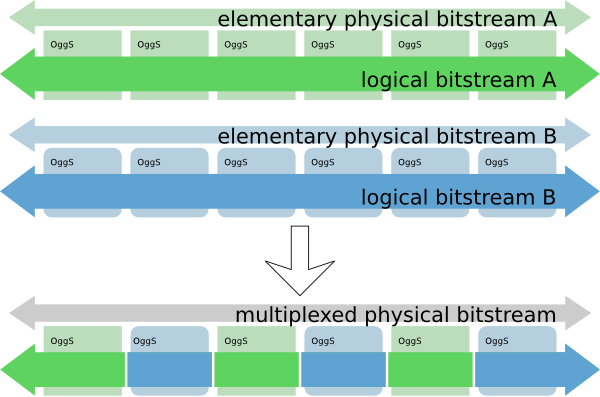
\includegraphics[width=8cm]{data/multiplex1.png}
\end{center}

The max size of a physical page is nearly 2$^{14}$ B, compared to 2$^{18}$ B of BT chunck.
So I define the granularity of spliting interval is 2$^{4}$ = 16 pages each chunck.
In general, the size of each chunks is dynamic, cause the size of each page are different, but 16 pages will buildup a typical chunck. However, no matter what the size of each chunck is, the SHA-1 of chunck data is always 160 B, that is the trick point of the design.

Refer to the infrastructure of metadata I provided before, after parsing the meta content, the SHA-1 value of each chunck will be stored in both a vector and buffer map.
After the vector was initalize,the content of the vetor would be constant, espically the order of the vector.
Because the order of vector should be the original order of video file spliting, we need to refer to the vector to recompse the \emph{OGG} bitstream.
The usage of the buffer map is to store the chuncks that low level swarming engine gethered from the internet.

}

\subsection{Buffer and Cache}
{
Usually the resource to feed codec is stored on the local disk which can be easily randomly accessed by the read function provided by system call with a simple API.
I have anaylsed the implementation of \emph{OGGPlayer} deeply.
While reading flat video file in local disk, there is a buildin ring buffer to store the data for synchronization.

The data structure of the buffer showed as followed:
\begin{lstlisting}[frame=tb]{}
typedef struct {
  void   ** buffer_list;
  void   ** buffer_mirror;
  int       buffer_size;
  int       last_filled;
  int       last_emptied;
  semaphore frame_sem;
} OggPlayBuffer;
\end{lstlisting}
In the buffer construction phase, the two level pointer ``buffer\_list will alloc a appointed size, the iterator last\_filled and 

%The buffer with a default size 20 B which 

\begin{center}
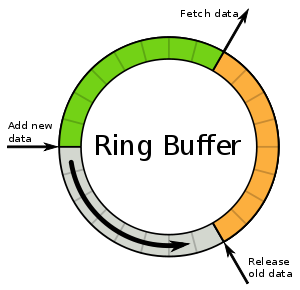
\includegraphics[width=5cm]{data/Ringbuffer.png}
\end{center}  

}


%include all chapters here
\chapter{Conclusions}
\label{conclusions}

Write your conclusions here. Typically 1-2 paragraphs where you tell
what was the problem and how it was solved. Then the main results in
1-2 paragraphs or possibly as a list. In addition, you can describe 
topics for future research in the last paragraph.

\newpage
%include appendexes here
%Appendixes do not have section numbers, but they are listed in the table 
%of contents:
\section*{Appendix A: OGG Glossary and Abbreviations}
\label{appendixa}
\addcontentsline{toc}{chapter}{Appendix A: OGG Glossary and Abbreviations}

   \hspace{1cm}bos page: The inital page ( beginning of stream) of a logical bitstream 
       which contains information to identify the codec type and other decoding-relevant infomation.

   chaining (or sequential multiplexing): Concatenation of two or more
      complete physical Ogg bitstreams.

   eos page: The final page (end of stream) of a logical bitstream.

   granule position: An increasing position number for a specific
      logical bitstream stored in the page header.  Its meaning is
      dependent on the codec for that logical bitstream and specified in
      a specific media mapping.

   grouping (or concurrent multiplexing): Interleaving of pages of
      several logical bitstreams into one complete physical Ogg
      bitstream under the restriction that all bos pages of all grouped
      logical bitstreams MUST appear before any data pages.

   lacing value: An entry in the segment table of a page header
      representing the size of the related segment.

   logical bitstream: A sequence of bits being the result of an encoded
      media stream.

   media mapping: A specific use of the Ogg encapsulation format
      together with a specific (set of) codec(s).

   (Ogg) packet: A subpart of a logical bitstream that is created by the
      encoder for that bitstream and represents a meaningful entity for
      the encoder, but only a sequence of bits to the Ogg encapsulation.

   (Ogg) page: A physical bitstream consists of a sequence of Ogg pages
      containing data of one logical bitstream only.  It usually
      contains a group of contiguous segments of one packet only, but
      sometimes packets are too large and need to be split over several
      pages.

   physical (Ogg) bitstream: The sequence of bits resulting from an Ogg
      encapsulation of one or several logical bitstreams.  It consists
      of a sequence of pages from the logical bitstreams with the
      restriction that the pages of one logical bitstream MUST come in
      their correct temporal order.

   (Ogg) segment: The Ogg encapsulation process splits each packet into
      chunks of 255 bytes plus a last fractional chunk of less than 255
      bytes.  These chunks are called segments.

%\input{appendixB.tex}

%The following adds references to the table of contents

\addcontentsline{toc}{chapter}{References}

%Give the name of your bibtex database, here it is dbase.bib
\bibliographystyle{plain}
\bibliography{refs.bib}
%\cite{P2PVideoStreaming}
%If you do not want to use bibtex, comment the previous and uncomment 
%the following, where references.tex contains the references:
%\input{references}


% Stop your text
%\end{CJK}
\end{document}

